\documentclass[onecolumn, draftclsnofoot, 10pt, compsoc]{IEEEtran}
\usepackage{graphicx}
\graphicspath{{./figures/}}

\usepackage{url}
\usepackage{setspace}
\usepackage{multicol}
\usepackage{pdflscape}
\usepackage{pdfpages}
\usepackage{hyperref}
\usepackage{subfig}
\usepackage{caption}
\usepackage{geometry}
\geometry{textheight=9.5in, textwidth=7in}

% \overfullrule=2in

% 1. Fill in these details
\def \CapstoneTeamName{			Ground Station Software Team}
\def \CapstoneTeamNumber{		30}
\def \GroupMemberOne{			Christopher Pham}
\def \GroupMemberTwo{}
\def \GroupMemberThree{}
\def \CapstoneProjectName{		OSU Robotics Club\\Mars Rover Ground Station}
\def \CapstoneSponsorCompany{	OSU Robotics Club}
\def \CapstoneSponsorPerson{	Nick McComb}



%Personal \newcommands

\newcommand{\functRequ}[4]{
\item #1%
\par
\begin{itemize}
\item \textit{Description:} #2.%
\item \textit{Rationale:} #3.%
\item \textit{Dependencies:} #4%
\end{itemize}
}



% 2. Uncomment the appropriate line below so that the document type works
\def \DocType{	%Problem Statement
				%Requirements Document
				Technology Review
				%Design Document
				%Progress Report
			 }
			
\newcommand{\NameSigPair}[1]{
  \par
  \makebox[2.75in][r]{#1} 
  \hfill
  \makebox[3.25in]{
      \makebox[2.25in]{\hrulefill} 
      \hfill
      \makebox[.75in]{\hrulefill}
  }
  \par\vspace{-12pt} 
  \textit{
      \tiny\noindent
      \makebox[2.75in]{} 
      \hfill
      \makebox[3.25in]{
          \makebox[2.25in][r]{Signature} 
          \hfill
          \makebox[.75in][r]{Date}
      }
  }
}
% 3. If the document is not to be signed, uncomment the command below
\renewcommand{\NameSigPair}[1]{#1}

%%%%%%%%%%%%%%%%%%%%%%%%%%%%%%%%%%%%%%%
\begin{document}
\begin{titlepage}
	\pagenumbering{gobble}
	\begin{singlespace}
		% 4. If you have a logo, use this includegraphics command to put it on the coversheet.
        \begin{minipage}{7in}
			\centering
			\hspace*{-.7in}
			$\vcenter{\hbox{
\includegraphics[height=4cm]{Oregon_State_College_of_Engineering_Logo}}}$
			\hspace*{.2in}
			$\vcenter{\hbox{
\includegraphics[height=2.5cm]{OSURCLogoOrange}}}$
		\end{minipage}

		\par\vspace{.35in}
		\centering
		\scshape{
			\huge CS Capstone \DocType \par
			{\large\today}\par
			\vspace{.5in}
			\textbf{\Huge\CapstoneProjectName}\par
			\vfill
			{\large Prepared for}\par
			\Huge \CapstoneSponsorCompany\par
			\vspace{5pt}
			{\Large\NameSigPair{\CapstoneSponsorPerson}\par}
			{\large Prepared by }\par
			Group\CapstoneTeamNumber\par
			% 5. comment out the line below this one if you do not wish to name your team
			\CapstoneTeamName\par 
			\vspace{5pt}
			{\Large
				\NameSigPair{\GroupMemberOne}\par
				\NameSigPair{\GroupMemberTwo}\par
				\NameSigPair{\GroupMemberThree}\par
			}
			\vspace{20pt}
            \begin{abstract}
            This document examines the differences between three technologies in three different subjects.
            Python GUI frameworks are going to be used on the project to show and abstract information coming from the rover towards the end user.
            The arm and graphical visualizers will be used to show how an object or the rover's state.
            Mapping software is going to be needed for any autonomy or any view of dangers on the map.
            This document goes over these different subjects and reviews technologies that will be suited for the system.

		\end{abstract}
		}
	\end{singlespace}
\end{titlepage}
\newpage
\pagenumbering{arabic}
\tableofcontents
\clearpage

% 8. now you write!
\section{Introduction}
My section of the technology review document is going to revolve around the "graphical" side of the ground station software. 
\section{Python GUI Frameworks}
\subsection{Overview}
A graphical user interface (GUI) is used by a program to obscure and allow the user to access and interact with objects instead of a command line interface system.
The GUI allows for people to interact with the system even if they are not trained.
A GUI framework is a pack of tools that will build a GUI using a commands and bindings and will allow for bindings across many systems like Linux, OS X, Windows, Android, and iOS.
A framework also comes with an added benefit of being made and maintained by the public or a company instead of being made in-house.

\subsection{Criteria}
Given the restrictions at the request of our client, I've chosen to focus more towards Python based implementations of graphical user interfaces. 
Some potential choices can be used in other languages but that is not a main focus point of this project.
The interface needs to be able to go into full-screen and needs to be able to change the colors of the GUI itself to a darker theme.
It also needs to support many video streams.

\subsection{Potential Choices}
\subsubsection{PyQT}
PyQt is a set of bindings for Python for the GUI framework Qt developed by The Qt company. \cite{PyQt}
PyQt can run on any platform that can support Qt like Windows, OS X, Linux, iOS, and Android.
Qt is not just a GUI toolkit, but also comes with "abstractions of network sockets, threads, Unicode, regular expressions, SQL databases, SVG, OpenGL, XML, a fully functional web browser, a help system, a multimedia framework, as well as a rich collection of GUI widgets." \cite{PyQt}
Qt also includes a designer called Qt Designer and PyQt is able to generate Python code from it.

\subsubsection{Tkinter}
Tkinker is GUI framework that is included in any Python 2 or 3 installation package.
Tkinker itself is a wrapper on top of the Tcl/Tk package from ActiveState. \cite{Tkinker}
Tkinker supports "most Unix platforms, as well as on Windows systems". \cite{Tkinker}
Tcl/Tk comes with a BSD-like license that allows for commercial use of their framework.

\subsubsection{Kivy}
Kivy is an open source framework for Python that is under MIT license. \cite{Kivy}
Kivy runs on Linux, Windows, OS X, Android, iOS and can use the same code for all platforms.
It can natively use most inputs and devices including "WM\_Touch, WM\_Pen, Mac OS X Trackpad and Magic Mouse, Mtdev, Linux Kernel HID, TUIO". \cite{Kivy}
Kivy also includes hardware acceleration using OpenGL ES 2.

\subsection{Comparison}
With all these frameworks, Tkinker/(Tcl/Tk) and PyQt/(Qt) are also possible on other languages using some other wrappers, unlike Kivy.
However, unlike the other frameworks, which are built in C or C++, Kivy is natively built in Python.
All the frameworks support OpenGL contexts (windows/frames) only PyQt and Kivy support OpenGL acceleration on the menus which might be necessary for how many video streams we are pushing.
Kivy in contrast to the other frameworks also supports multi-touch enabled devices like phones, and tablets unlike the other frameworks.
Tkinker however is included in all builds of Python released, making it very easy for quick and lightweight programming and prototyping compared to other frameworks.
Qt requires payment for any commercial product, unlike the others.

\subsection{Decision}
My suggestion for this project would be PyQt.
PyQt's fee that Qt asks for is not applied to this project.
PyQt and Qt in general have good support and documentation because its longevity, numerous tutorials, and support by the community.
Kivy would work well for the project if it had more documentation but its OpenGL rendering would be fantastic for design ideas we have.
Kivy is also built more towards multi-input systems which is not our focus.
Tkinker would work well for small projects but the lack of OpenGL acceleration might be questionable for the all the video streams that might be handled on the system.

\section{Arm/Graphical Visualization}
\subsection{Overview}
For this project, one important aspect is going to be visualizing how the arm is currently moving in respect to the rover itself and showing how the user input changes the arm visually.
The need comes from the integration between our project and the other senior project that revolves around the rover arm.
Without the visualization, the other senior project can not test to see if their arm works correctly on the rover and for later competition usage. 

\subsection{Criteria}
If this was to be made using the command line or via text, it would be very confusing.
Per requests, the arm visualizer needs to resemble the arms.
The other requirements would be needing to able to run on Linux (Ubuntu) and easy integration with the ROS (Robot Operating System) on the Rover. 

\subsection{Potential Choices}
\subsubsection{ROS Visualization}
Inbuilt into ROS, there is a package called rvis which allows for the system to visualize objects using displays.
The included displays in rvis are \cite{rvis}:
\begin{center}
\begin{tabular}{c c c c}
Axes & Effort & Camera & Grid \\
Grid Cells & Image & Interactive Marker & Laser Scan \\
Map & Markers & Path & Point \\
Pose & Pose Array & Point Cloud (two types) & Polygon \\
Odometry & Range & RobotModel & TF \\
& Wrench & Oculus & \\
\end{tabular}
\end{center}
The package is also very well documented with sample code and projects to show how some interactions happen.

\subsubsection{OpenGL visualization}
We can build a system using one of our GUI frameworks to give us access to an OpenGL window.
In that window, we can then write to it using some OpenGL and Python code to form the arm. 
We can use any shapes we want like line pieces or even importing the arm's 3D model and modifying it from there. 
Inverse kinematics is needed to get the joints working correctly if the arm is moving from point to point, and normal kinematics to get the final location from arm segment movements.
We would be able to control how fast the video/render would be refreshing, drawing, or rendering size which would allow for granularity control to reduce CPU or GPU usage.

\subsubsection{Moveit Simulator}
We could also use simulator software that can take the signals from the inputs/joysticks and then send them both to the rover and simulator.
The simulator can emulate what the arm SHOULD do and can be imported from the other senior project that is already simulating the arm using the same software.
The video can be captured using OpenCV or open source prorgrams like Istanbul to stream the video to the GUI.

\subsection{Comparison}
Compared to ROS and OpenGL, Moveit actually just emulates the arm while the others calculate how the arm should move using inverse kinematics.
ROS has all built-in displays in which many other things like mapping software and waypoint systems would be much simpler than building our own system for the project.
OpenGL provides flexibility compared to the others but does not include any built-in packages or anything of the sort.

\subsection{Decision}
I think that the visualization should be a mix of ROS and some custom OpenGL.
The combination of the two allow for access to packages that are included and built around ROS while also including the flexibility that is included with OpenGL. 
The arm can be visualized using the included packages like rvis, but other things like the IMU (Inertia Measurement Unit) might be hard to visualize in rvis and would be possible with custom OpenGL code.

\section{Mapping Software}
\subsection{Overview}
Another part of the project is the mapping system.
In competition, the Robotics team wishes to see where the rover is currently on the map.
We are going off the assumption that the way-point system needs to be built, but we can use a package to deal with the GPS location and mapping.

\subsection{Criteria}
A requirement would be ease of integration between the rover and ground station.
Another would be the ability to use the mapping software with a reasonable amount of delay or no Internet at all.

\subsection{Potential Choice}
\subsubsection{ROS Packages}
There are inbuilt packages for GPS and GPS location parsing in the ROS subsystem.
Using packages like rvis or mapviZ can display the map and transform the map image to display the correct location.
The location can be calculated on the rover or on the ground control system.

\subsubsection{Google Maps/Earth}
Using the same packages as above, instead of parsing the location on the robot or ground control system, the rover/ground station can parse the information given to it by sending it to Google.
This would remove any need for calculating location at all and the map would be generated by Google.

\subsubsection{Custom Mapping/Packages}
We could build a system using our own polling and parsing of the GPS information.
This can be represented by texture location using an external package like Kartograph \cite{karto} for Python.
Kartograph can then return an SVG (Scalable Vector Graphics) which can be displayed on the GUI.


\subsection{Comparison}
ROS and Google are very similar with the only differentiating thing about the two would be where the information being sent, locally or via ground control to a remote server.
ROS and the custom software are very similar but uses in-house code or open source code.
The only difference between all of these is how the GPS data is analyzed and texture map is generated and then put onto the screen.
\begin{figure}[h]
\centering
\subfloat[Map Visualization Using Mapviz Package \cite{mapviz}]{\label{ref_label1}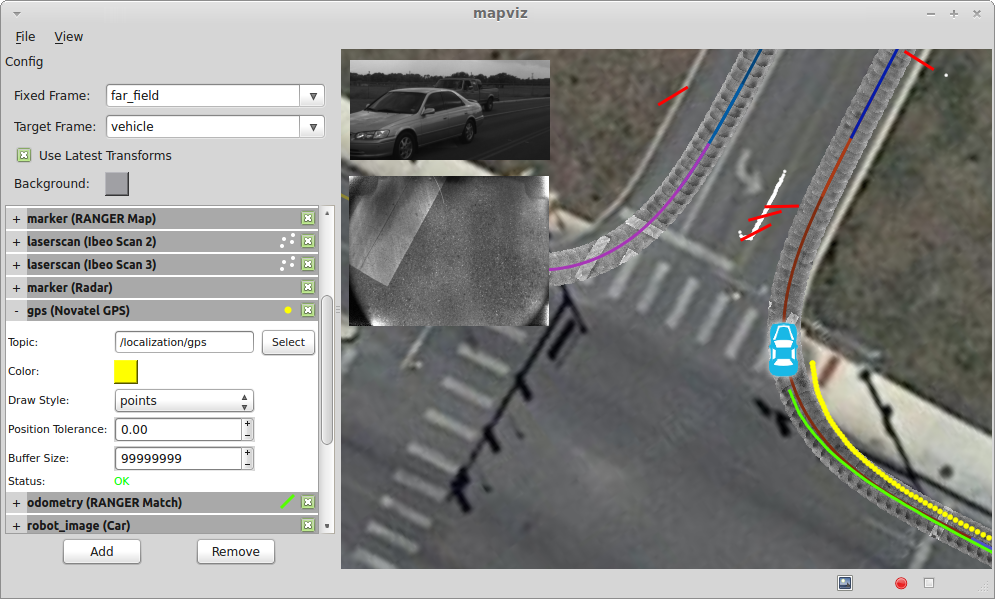
\includegraphics[width=0.33\textwidth]{mapviz}}
\subfloat[Google Maps using Decimal Degrees]{\label{ref_label2}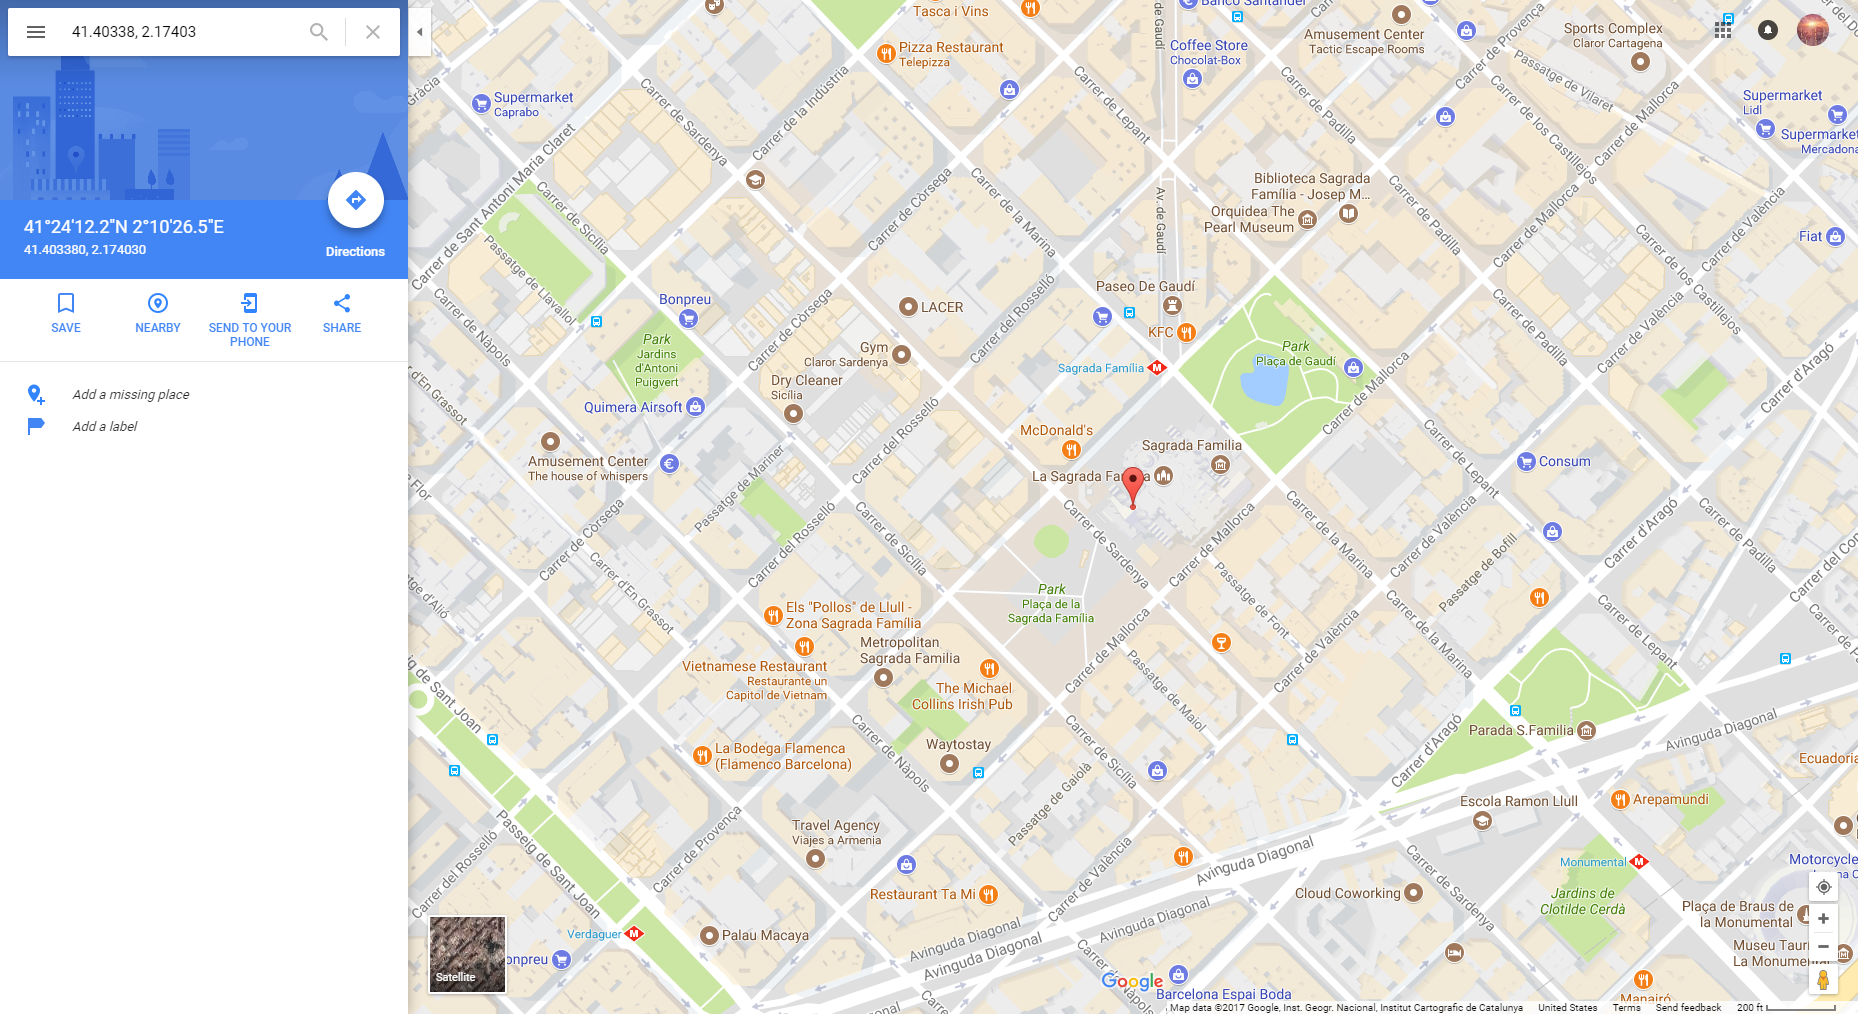
\includegraphics[width=0.33\textwidth]{chrome_2017-11-21_13-32-08}}
\subfloat[Kartograph Render \cite{karto}]{\label{ref_label3}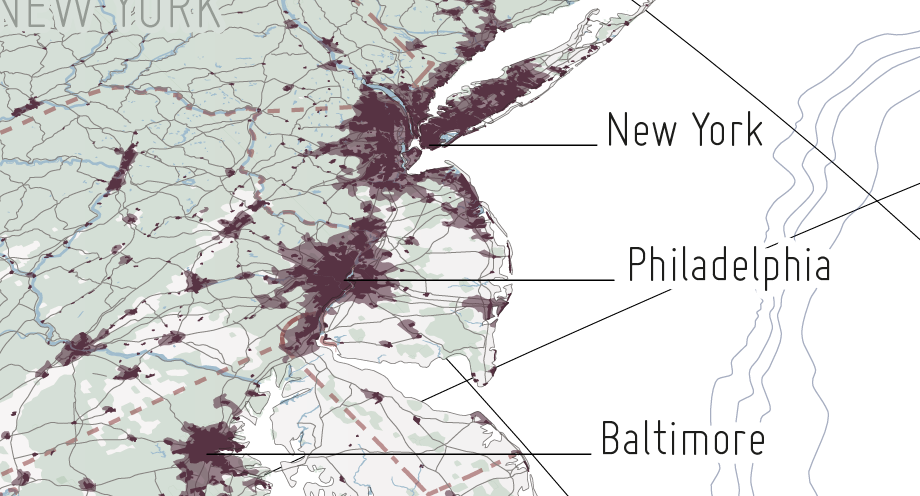
\includegraphics[width=0.33\textwidth]{detail}}
\captionsetup{justification=centering}
\centering\caption{Map Visualization}
\end{figure}

\subsection{Decision}
I think that the project should use the ROS packages because all of those are open source and packages are constantly made for problems like this.
ROS also has integrations between other packages like rvis and mapping software.
And in the environment where the competition is going to take place, the speed and the Internet quality might be sub-par and any external requests would make the system react very slowly or be completely off.
Another problem with using Google would be that we can not use their mapping system to do anything autonomous as stated from their ToS (Terms of Service) and we would need to use some other system like OpenSourceMaps. 
If we had to build a custom solution to this project, Kartograph would be good.
Kartograph produces SVG files which Qt takes for but the lack of documentation might make building the project longer than alloted.

\begin{thebibliography}{9}
\bibitem{PyQt}\href{https://riverbankcomputing.com/software/pyqt/intro}{"What is PyQt." Riverbank Computing Limited. November 2017}
\bibitem{Tkinker}\href{https://docs.python.org/2/library/tkinter.html}{"Tkinker -- Python interface to Tcl/TK" Python Software Foundation. November 2017}
\bibitem{Kivy}\href{https://kivy.org/}{"Kivy." Kivy Organization. November 2017}
\bibitem{rvis}\href{http://wiki.ros.org/rviz/DisplayTypes}{"rvis/DisplayTypes" David Gossow. August 17, 2013}
\bibitem{mapviz}\href{https://github.com/swri-robotics/mapviz}{"Mapviz." swri-robotics, November 21, 2017}
\bibitem{karto}\href{http://kartograph.org/}{"Kartograph - A Simple and lightweight frameowkr for createing interavtive vector maps"}
\end{thebibliography}
\end{document}